\documentclass[UTF8,a4paper]{ctexart}
\usepackage[utf8]{inputenc}
\usepackage{amsmath}
\usepackage{pdfpages}
\usepackage{graphicx}
\usepackage{wrapfig}
\usepackage{listings}
\title{线控作业1}
\author{张蔚桐\ 2015011493\ 自55}
\begin {document}
\maketitle
\section{}
\section{}
从图\ref{f1ori}中可以预计,系统的传递函数可以表示为$G(s)=\frac{K}{s(T_1s+1)(T_2s+1)},T_1>0,T_2>0$可以根据相频图估计转折频率$\omega_1=18.14\rm{rad/s},\omega_2=1103\rm{rad/s}$可得$T_1=\frac{1}{\omega_1}=0.551\rm{s},T_2=\frac{1}{\omega_2}=0.9066\times 10^{-3}\rm{s}$,同时,考虑辐频在$\omega=1\rm{rad/s}$附近的增益可得$20lg(K)=-9.2;K=0.346$因此系统传递函数可以表示为$$G(s)=\frac{0.346}{s(0.551s+1)(0.9066\times 10^{-3}s+1)}$$,对应的Bode图如图\ref{f1the}所示,可以看出和实际bode图\ref{f1ori}还是基本符合的
\begin{figure}
\centering
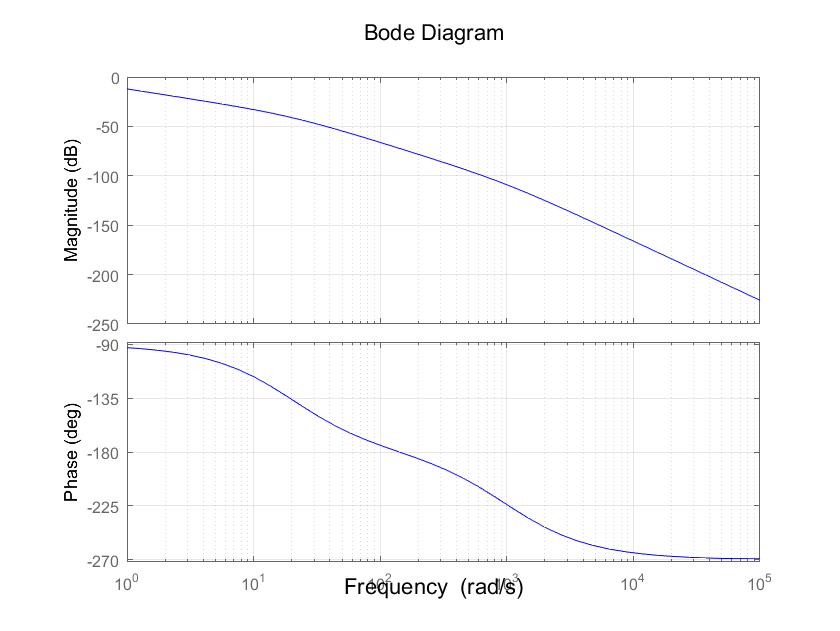
\includegraphics[width=\textwidth]{motorG.jpg}
\caption{原图像}
\label{f1ori}
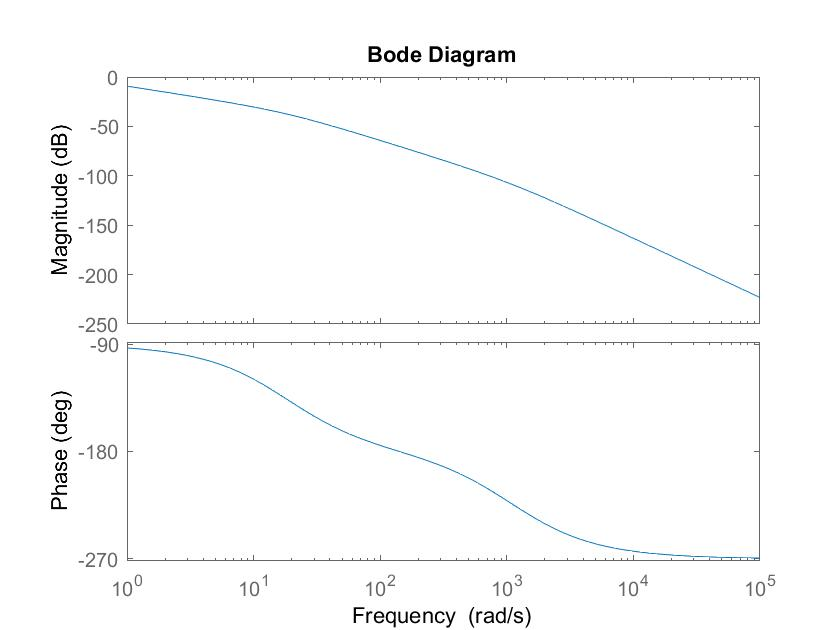
\includegraphics[width=\textwidth]{RmotorG.jpg}
\caption{理论图像}
\label{f1the}
\end{figure}
\section{}
如图\ref{f2ori}显然这是一个惯性环节的图像,可以直接看出$$G(s)=\frac{0.102}{(0.001s+1)}$$MATLAB仿真之后的图像如图\ref{f2the}所示,和原图\ref{f2ori}基本一致
\begin{figure}
\centering
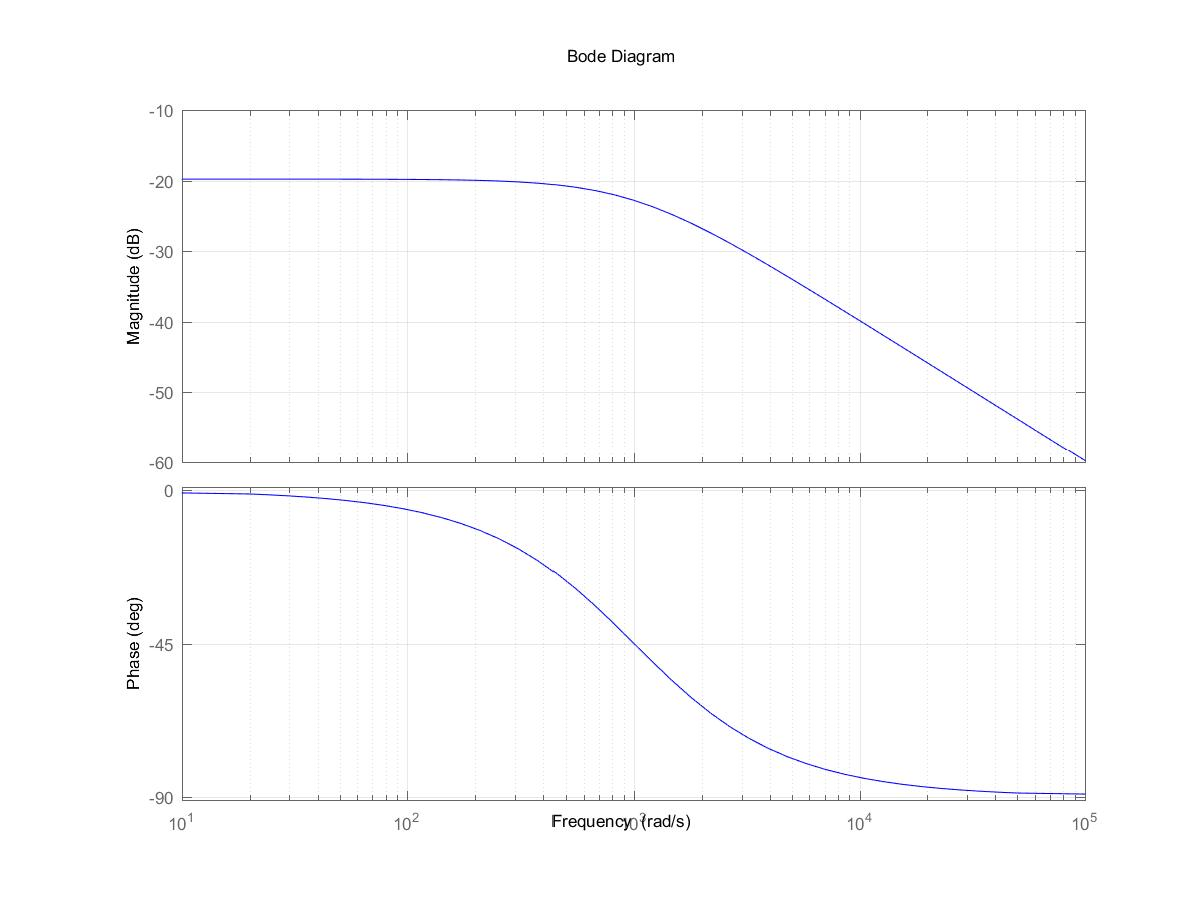
\includegraphics[width=\textwidth]{motorG1.jpg}
\caption{原图像}
\label{f2ori}
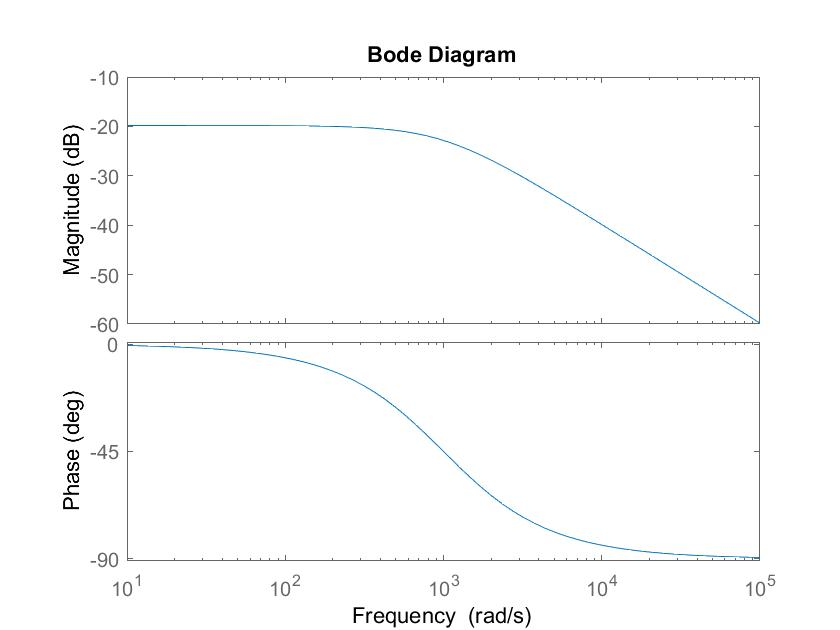
\includegraphics[width=\textwidth]{RmotorG1.jpg}
\caption{理论图像}
\label{f2the}
\end{figure}
\section{}
可以看出系统的传递函数为$G(s)=\frac{K}{s(Ts+1)},T>0$,并由图\ref{f3ori}可以得到$20lg(K)=7.196,K=2.29,T=\frac{1}{20}=0.05$因此$$G(s)=\frac{2.29}{s(0.05s+1)}$$MATLAB作图如图\ref{f3the}所示,和实际情况相差不多
\begin{figure}
\centering
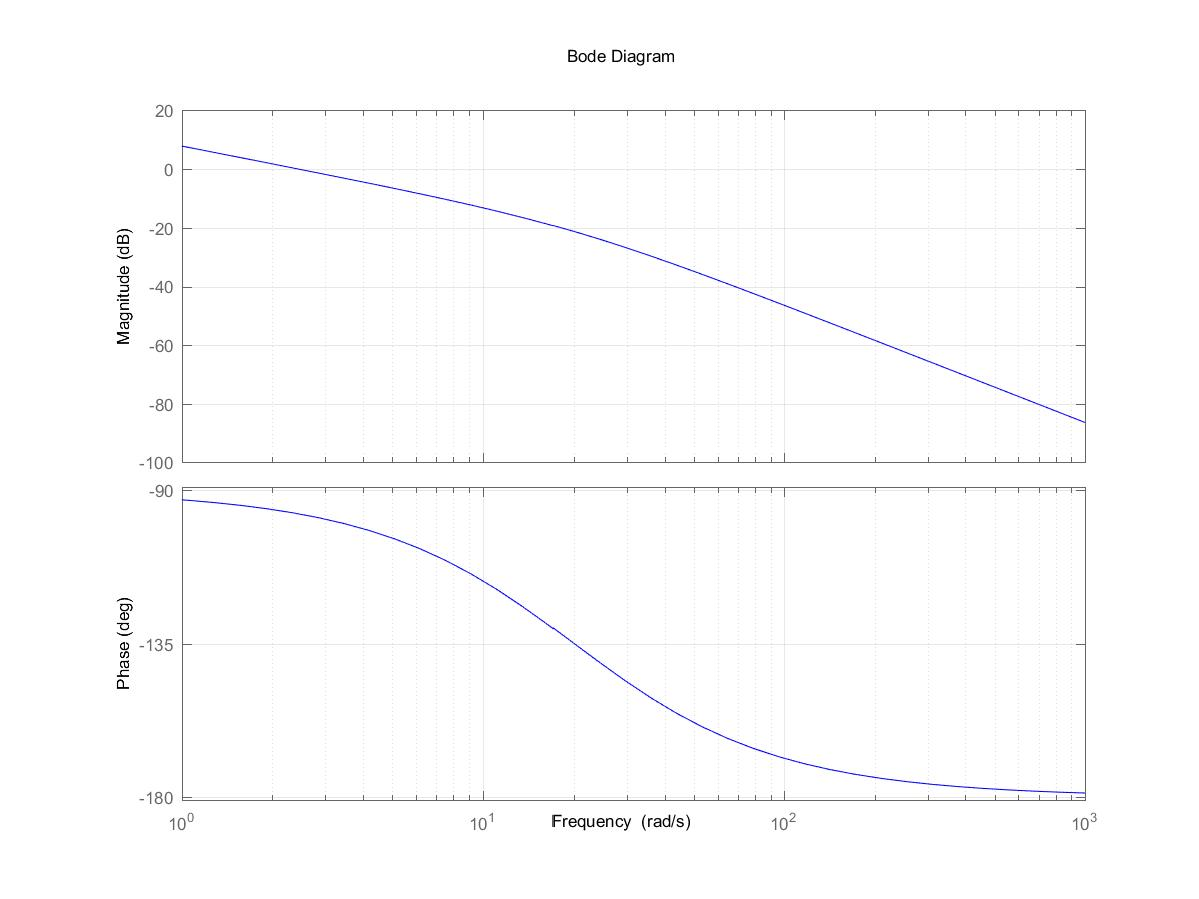
\includegraphics[width=\textwidth]{motorG2.jpg}
\caption{原图像}
\label{f3ori}
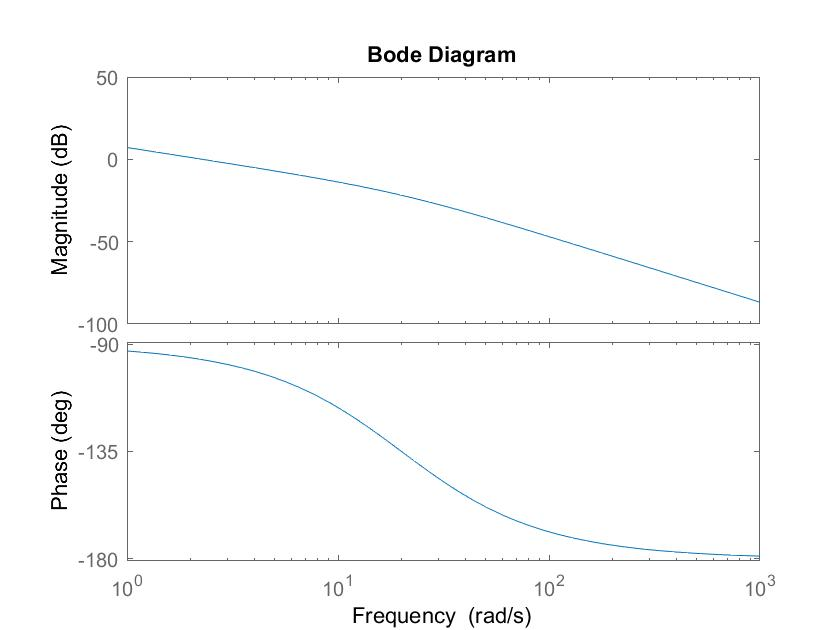
\includegraphics[width=\textwidth]{RmotorG2.jpg}
\caption{理论图像}
\label{f3the}
\end{figure}
\section{}
根据KCL,KVL,可以得到
$$\begin{cases}
\dot{x_3}=\frac{1}{C_3}x_4 \\
\dot{x_4}=-\frac{1}{L_1}x_1-\frac{1}{L_1}x_3+\frac{1}{L_1}u \\
\dot{x_2}=-\frac{1}{C_2R}x_1-\frac{1}{C_2R}x_2+\frac{1}{C_2R}u \\
\dot{x_1}=\frac{1}{C_1}x_4-\frac{C_2}{C_1}\dot{x_2} = \frac{1}{C_1R}x_1+\frac{1}{C_1R}x_2+\frac{1}{C_1}x_4-\frac{1}{C_1R}u
\end{cases}$$
并进一步得到$$y=RC_2\dot{x_2}=-x_1-x_2+u$$因此得到
$$\begin{cases}

\mathbf{A}=\begin{pmatrix}
\frac{1}{RC_1} & \frac{1}{RC_1} & 0 & \frac{1}{C_1} \\
-\frac{1}{RC_2} & -\frac{1}{RC_2} & 0 & 0 \\
0 & 0 & 0 & \frac{1}{C_3} \\
-\frac{1}{L_1} & 0 & -\frac{1}{L_1} & 0
\end{pmatrix} \\ 
\\ 
\mathbf{b}=\begin{pmatrix}
-\frac{1}{RC_1} &
\frac{1}{RC_2} &
0 &
\frac{1}{L_1}
\end{pmatrix}^\mathbf{T}\\
\\ 
\mathbf{c}^\mathbf{T}=\begin{pmatrix}
-1 & -1 & 0 & 0 \end{pmatrix}\\
\\ 
\mathbf{d}=\begin{pmatrix} 1 \end{pmatrix}
\end{cases}$$
\section{}
由泊肃叶定律,可以得到状态方程为 $$\begin{cases}
c_1x_1=u_1+\frac{\rho g}{R_2}x_2-\frac{\rho g}{R_2}x_1-\frac{\rho g}{R_1}x_1 \\
c_2x_2=u_2-\frac{\rho g}{R_2}x_2+\frac{\rho g}{R_2}x_1\end{cases}$$
输出方程为$$y=\frac{\rho g}{R_1}x_1$$其中$\rho$是液体的密度,$g$是重力加速度
\section{}
记滑块1的位置为$F_1$滑块2的位置为$F_2$,由牛顿第二定律得
\section{}
\section{}
\section{}
\section{}
\section{}
\section{}
\section{}
\section{}
\section{}
\section{}
\end{document}